\newpage
\section{Auswertung}
\label{sec:Auswertung}

Welche Programme verwendet?

\subsection{Eichung des Elektromagneten}
\label{sec:AuswEichung}

\input{build/eichung.tex}

\begin{figure}
	\centering
	\includegraphics[height=8cm]{build/eichung.pdf}
	\caption{Aufgenommene Werte der magnetischen Flussdichte in Abhängigkeit des
	anglegten Stroms mit durchgängig dargestellter Regression.}
	\label{fig:eichung}
\end{figure}


\subsection{Analyse der roten Spektrallinie}
\label{sec:AuswRot}

\begin{figure}
	\centering
	\includegraphics{images/termschema-rot.pdf}
	\caption{Termschema für die rote Linie der \ce{Cd}-Lampe.}
	\label{fig:termschema-rot}
\end{figure}


\subsection{Analyse der blauen Spektrallinie}
\label{sec:AuswBlau}

\begin{figure}
	\centering
	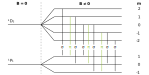
\includegraphics{images/termschema-blau.pdf}
	\caption{Termschema für die blaue Linie der \ce{Cd}-Lampe.}
	\label{fig:termschema-blau}
\end{figure}
